
\chapter{Wykorzystane zasoby sprzętowe i technologie}
\section{Kamera termowizyjna Lepton}

\begin{figure}[h]
    \centering
    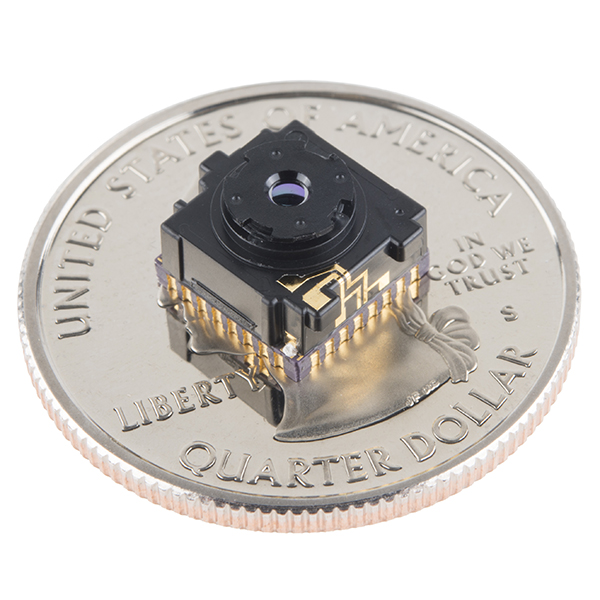
\includegraphics[width=0.6\textwidth]{images/Lepton}
    \caption{Widok poglądowy na kamere Flir Lepton.}
    \label{fig:lepton}
\end{figure}
 
Lepton jest zintegrowaną w pojedynczym układzie kamerą składającą się z soczewki, sensora podczerwieni fal długich (ang. LWIR – long wave infrared) oraz elektroniki sterującej i przetwarzającej sygnał. Checuje siębardzo małymi wymiarami co czyni go idealnym do zastosowań mobilnych. Układ ma możliwość domontowania dodatkowej przesłony która jest wykorzystywana do automatycznej optymalizacji procesu ujednolicania obrazu (kalibracji sensora).
Prosty do integracji z dowolnym mikrokontrolerem dzięki zastosowaniu standardowych protokołów i interfejsów. Lepton po podłączeniu od razu pracuję w domyślnym trybie pracy, który może zostać zmieniony za pomocą CCI (ang. camera control interface – interfejs kontroli kamery).\cite{lepton}
Parametry:
\begin{itemize}
\item Wymiary: 11,8 x 12,7 x 7,2 mm, 
\item Sensor: niechłodzony mikrobolometr VOx (tlenek wanadu),
\item Rejestrowany zakres: fale długie podczerwieni, 8$\mu m$ do 14$\mu m$ ,
\item Wielkość piksela: 17 $\mu$m,
\item Rozdzielczosć: 80x60 pikseli,
\item Ilość klatek na sekundę 8,6,
\item Zakres rejestrowanych temperatur: -10  $^\circ$  C 140  $^\circ$  C (Tryb wysokiego wzmocnienie),
\item korekta niejednorodności matrycy: automatyczna na bazie przepływu optycznego
\item kąt widzenia horyzontalny / diagonalny: 51 $^\circ$ \\ 66 $^\circ$,
\item Głębia ostrości: od 10cm do nieskończoności
\item Format wyjściowy: do wyboru: 14-bit, 8-bit (z AGC (ang. automatic gain control – automatyczna kontrola wzocnienia)) 24-bit rgb (z ACG i koloryzacją).
\item Interfejs video: VoSPI (Video over Serial Peripherial Interface)
\item Interfejs sterujący: CCI (I2C podobny)
\end{itemize}
\section{Zynq-7000}

Rodzina układów Zynq-7000 bazuje na architekturze SoC (ang. System on Chip). Posiadają zintegrowany kompletny system składający podzielonego na dwie części: systemu procesorowego bazującego na procesorze ARM Cortex-A9 (PS ang. Porcessing System) oraz logikę programowalną (PL ang. programable logic) FPGA w jednym układzie scalonym. Na rysunku \ref{fig:zynq7000} przedstawiono schemat architektury. Prócz procesora cześć procesorowa posiada wbudowaną pamięć, kontroler pamięci zewnętrzne oraz szereg interfejsów dla układów peryferyjnych takich jak USB, GigEthernet, CAN, I2C, SPI. W części logiki programowalnej znajdują się bloki logiki konfigurowalnej (CLB ang. configurable logic block), 36Kb bloki pamięci RAM, procesory sygnałowe DSP48, układ JTAG, układy zarządzania zegarami oraz dwa 12-bitowe przetwornik analogowo-cyfrowy.

Komunikacji między częścią procesorową a logiką programowalną odbywa się za pośrednictwem Interfejsu AXI (ang. Advanced Extensible Interface), oraz bezpośrednio wykorzystując porty generalnego przeznaczenia, przerwania, oraz poprzez bezpośredni dostęp do pamięci (DMA ang. Direct Memory Access) 

\begin{figure}[h]
    \centering
    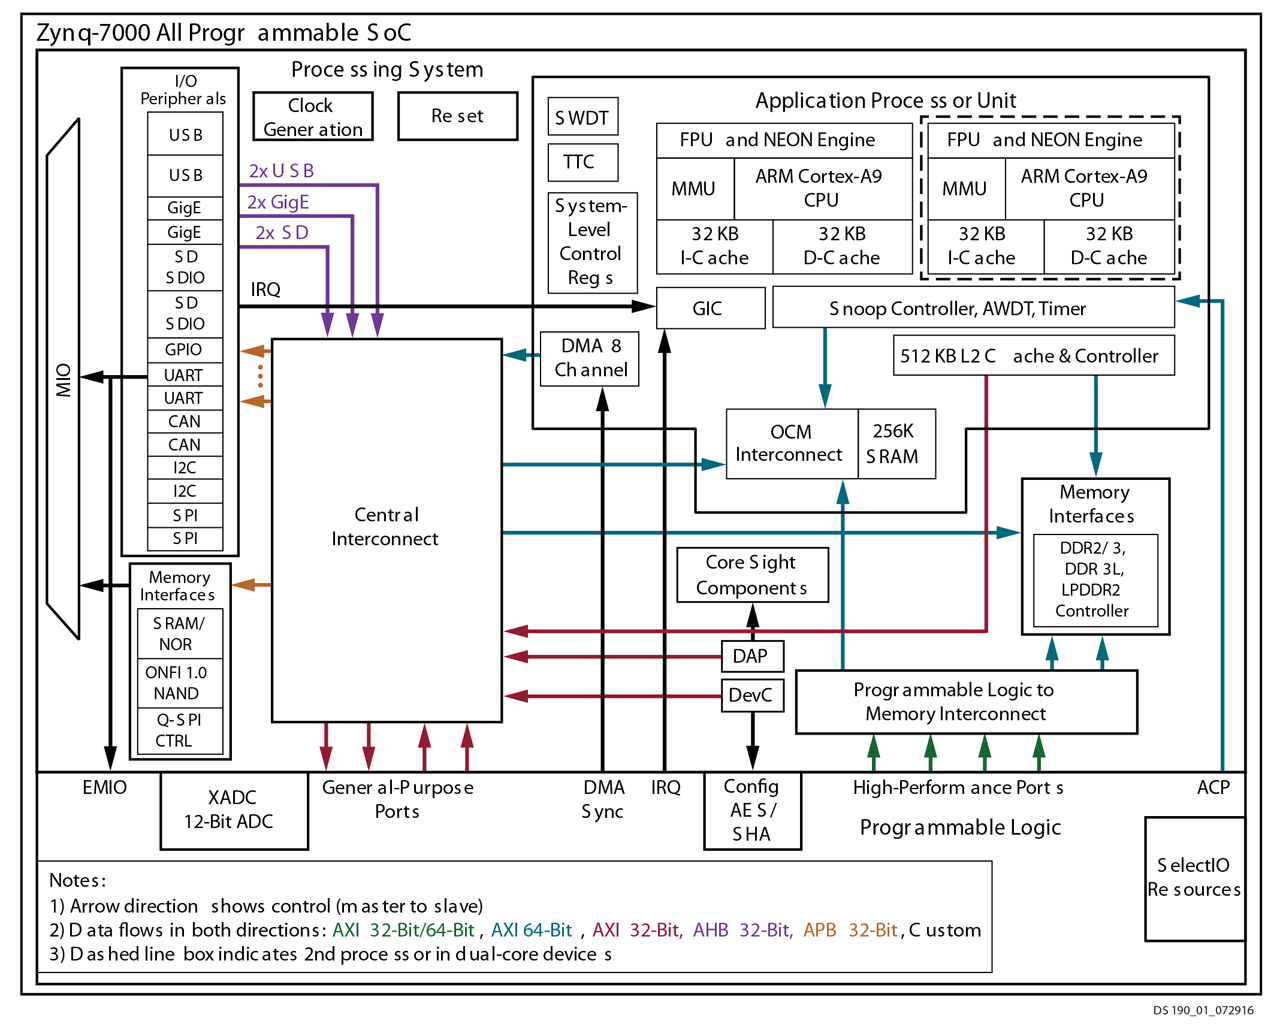
\includegraphics[width=1\textwidth]{images/Zynq-7000-Overview}
    \caption{Schemat ogólny architektury układu Zynq-7000.}
    \label{fig:zynq7000}
\end{figure}

\section{Interfejs AXI}
 AXI (ang. Advanced eXtensible Interface zawansowany rozszerzalny interfejs) jest częścią ARM AMBA (ang. Advanced Microcontroller Bus Architecture) – otwartego standardu, specyfikacją do zarządzania i połączeń między blokami funkcyjnymi w SoC. Aktualnie jest stosowana AMBA 4.0 która wprowadziła drugą wersję AXI, AXI4. Występują trzy typy interfejsów dla AXI4:
\begin{itemize}
\item AXI4 – stosowany w wysokowydajnych transferach w przestrzeni pamięci (ang. memory-mapped)
\item AXI4-Lite – stosowany dla prostszych operacji w przestrzeni pamięci (na przykład do komunikacji z rejestrami kontrolnymi i statusu)
\item AXI4-Stream – stosowany do wysokiej prędkości transmisji strumieniowych
\end{itemize}
Specyfikacja interfejsu zakłada komunikację pomiędzy pojedynczym AXI master i pojedynczym AXI slave, która ma na celu wymianę informacji pomiędzy tymi dwoma blokami funkcyjnymi IP core. Kilkanaście interfejsów AXI master i slave mogą zostać połączone między sobą za pomocą specjalnej struktury zwanej interconnect block (blok międzypołączeniowy) w której odbywa się trasowanie połączeń do poszczególnych bloków. 

AXI4 i AXI4-Lite składają się z 5 różnych kanałów:
\begin{itemize}
\item Kanał adresu odczytu,
\item Kanał adresu zapisu,
\item Kanał danych odczytanych
\item Kanał danych do zapisania
\item Kanał potwierdzenia zapisu
\end{itemize}
Dane mogą płynąć w obie strony pomiędzy master a slave jednocześnie. Ilość danych które można przesłać w jednej transakcji w przypadku AXI4 wynosi 256 transferów, zaś AXI4-Lite pozwala na tylko 1 transmisję.

AXI4-Stream nie posiada pola adresowego, a dane mogą być przesyłane nieprzerwanie. 
\section{Wykorzystanie AXI-Stream do transmisji sygnału video.} 
W odróżnieniu od klasycznej implementacji przetwarzania strumieniowego video, w AXI-Stream przesyłane są jedynie aktywne piksele. Linie synchronizacji poziomej i pionowej są odrzucane albo są połączane do specjalnego bloku detekcji timingów który mierzy parametry wchodzącego strumienia wizyjnego (ilość pikseli na linie, czas ilość aktywnych linii, czas wyciemnienia itd.). Podobnie informacje o synchronizacji są dodawane przez blok generujący timingi.

Do transmisji wykorzystane jest 6 linii: jedna linia danych i pięć kontrolno-sterujących. 
\begin{itemize}
\item Video Data – linia danych o szerokości jednego (albo dwóch) pikseli. Szerokość tej linii powinna być wielokrotnością liczby osim (16, 24, 48 itd.)
\item Valid – Linia podająca czy dane piksela są poprawne,
\item Ready – Linia kontrolna informująca urządzenie master że slave jest gotowy do transmisji danych,
\item Start Of Frame – linia która wskazuje pierwszy piksel nowej ramki,
\item End Of Line – linia wskazująca ostatni piksel w linii.
\end{itemize}
Aby mógł wystąpić poprawny transfer danych linie Valid i Ready muszą być w stanie wysokim podczas rosnącego zbocza zegara. Przykładowe nawiązanie transmisji przedstawia rysunek \ref{fig:handshake}

\begin{figure}[h]
    \centering
    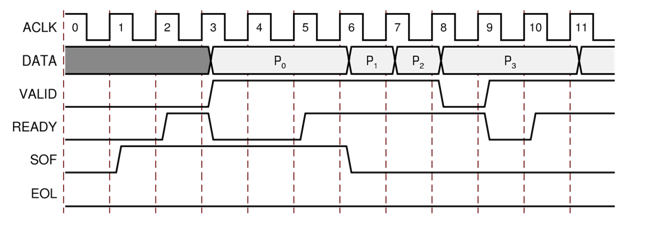
\includegraphics[width=1\textwidth]{images/axi-stream_hendshake}
    \caption{Przykład rozpoczęcia transmisji Reday/Valid.}
    \label{fig:handshake}
\end{figure}
